\section{Arquitectura}

En la figura \ref{fig:arquitectura} se muestra el diagrama de la arquitectura propuesta con la que se trabajara para solucionar la problemática.

%En la figura \ref{fig:arquitectura} se describirá la arquitectura propuesta para la solución de la problemática.

\begin{figure}[htb]
	\centering
	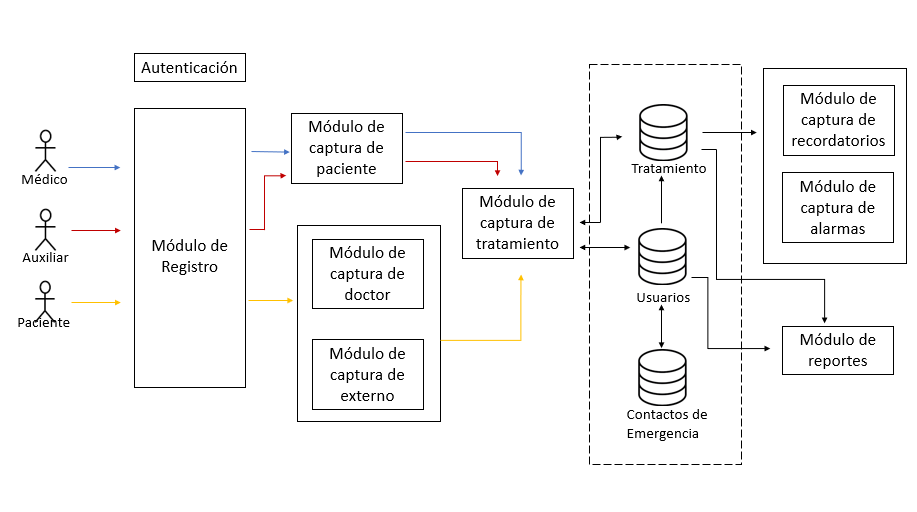
\includegraphics[width=0.8\textwidth]{images/cap2/Arquitectura}
	\caption{Arquitectura} \label{fig:arquitectura}
\end{figure}

Como podemos notar en la figura \ref{fig:arquitectura} se cuenta con cuatro actores que participaran en el sistema. Los cuales son :
\begin{itemize}
	\item Administrador: Dentro del sistema se le llama \textbf{Administrador} a la persona que esta encargada de ingresar los medicamentos a la base de datos, ya que estos serán los utilizados en los tratamientos del paciente.
	
	\item Paciente: Se le llama paciente a la persona que cuenta con un diagnostico generado por el \textbf{Médico} que se encuentra a cargo de su salud.\\
	Las acciones con las que cuentan son:
	\begin{itemize}
		\item Agregar el tratamiento medico.
		\item Modificar el tratamiento medico.
		\item Eliminar el tratamiento medico.
		\item Agregar médico.
		\item Modificar médico.
		\item Eliminar médico.
		\item Agregar externo.
		\item Modificar externo.
		\item Eliminar externo.
		\item Consulta de su tratamiento.
		\item Modificación de notificación.
		\item Agregar contactos de emergencia.
	\end{itemize}

	\item Médico: \\ \textbf{Médico} dentro del sistema es el profesional de la salud que se encarga del diagnostico del paciente y las acciones dentro del sistema son:
		\begin{itemize}
			\item consultar el total de pacientes que tiene.
			\item agregar un tratamiento medico a sus pacientes.
			\item modificar un tratamiento medico a sus pacientes.
			\item eliminar un tratamiento medico a sus pacientes.
			\item consultar el tratamiento medico de sus pacientes.
			\item consultar el historial medico de sus pacientes.
			\item agregar un paciente.
			\item modificar un paciente.
			\item eliminar un paciente.
		\end{itemize}

	\item Externo: El actor \textbf{Externo} nace de la necesidad de ayudar a los Pacientes que cuentan con poca o nula experiencia los dispositivos moviles o que por factores ajenas a la aplicación como son la de edad o alguna enfermedad les sea imposible utilizar la aplicación por si mismos\\
	Las acciones que tendra dentro de la aplicación son:
	\begin{itemize}
		\item Agregar Paciente.
		\item Modificar Paciente.
		\item Eliminar Paciente.
		\item Agregar Tratamiento medico.
		\item Modificar Tratamiento medico.
		\item Consultar Tratamiento medico.
		\item Modificar notificación
	\end{itemize}
\end{itemize}


\section{Módulos}
La arquitectura contara con los siguientes módulos:
\begin{itemize}
	\item Modulo de registro: Este modulo es el encargado de registrar e ingresar a los actores dentro de la aplicación. 
	
	
	\item Modulo de Autenticación: Una vez que te hayas registrado dentro de la aplicación, el modulo de autenticación se encargara de verificar tu perfil y habilitar los módulos correspondientes.
	
	 
	\item Modulo de captura de paciente: Este modulo es el encargado de agregar al paciente con el que trabajaran el doctor y el externo.
	
	\item Modulo de captura de doctor: Este modulo es el encargado de agregar al doctor que esta a cargo del tratamiento del paciente.
	
	\item Modulo de captura de externo: Este modulo es el encargado de agregar al externo que esta a cargo del tratamiento del paciente.
	
	\item Modulo de captura de tratamiento: Este modulo es el encargado de ingresar el tratamiento medico del paciente y con el que podrán trabajar tanto el doctor como el externo. 
%	y lo asociara al perfil del paciente con la información correspondiente del tratamiento.
	
	\item Módulo de recordatorios: Este modulo es el encargado de crear los recordatorios para tomar los medicamentos que se ingresaron en el tratamiento.
	
	\item Módulo de alarmas: Este modulo es el encargado de crear las alarmas cuando la situación del paciente sea delicada o que la toma de un medicamento sea de alta prioridad.
	
	\item Módulo de reportes: Este modulo es el encargado de generar un reporte con la información del tratamiento y datos relevantes del paciente como lo son la edad, estatura, peso, etc...
	
	
	
	
	
%	\item Módulo de Autenticación: El modulo encargado de verificar tu perfil y darte acceso a los módulos correspondientes.
%	\item Módulo captura de tratamientos: El modulo encargado de ingresar el tratamiento medico y lo asociara al perfil del paciente con la información correspondiente del tratamiento.
%	\item Módulo de recordatorios: Una vez que se paso por el modulo de \textbf{Captura de tratamiento} llegamos al modulo de recordatorios en donde se generaran los notificaciones a partir de la información obtenida del modulo de captura de tratamiento.
%	\item Módulo de alarmas: Este modulo es el encargado de cuando una notificación no haya sido silenciada esta se convierta en una alarma que le estará recordando al paciente tomar su medicamento.
%	\item Módulo de reportes: El modulo de reportes sirve para notificar al medico y al paciente que tan constante ha sido con su tratamiento.
%	\item Módulo de estadísticas: 
\end{itemize}


\section{Requerimientos}
Los requerimientos funcionales describen lo que el sistema debe hacer. Son declaraciones de los
servicios que debe proporcionar el sistema, de la manera en que este debe reaccionar a entradas.\\
particulares y de como se debe comportar en situaciones particulares.
En la siguiente sección se especificaran los requerimientos con los que estará trabajando la aplicación.\\

Requerimientos Funcionales:

\begin{itemize}
	\item RF1 - Registro de Usuario
	La aplicación permitirá el registro de nuevos usuarios mediante el ingreso de su nombre, correo electrónico y contraseña.
	
	\item RF2 - Acceso al Sistema.
	La aplicación permitira el acceso al sistema proporcionando el correo electrónico y la contraseña con la que se registraron en la aplicación
	
	Los usuarios accederán al sistema proporcionando el correo electrónico y la contraseña con la que se registraron en la aplicación
	
	\item RF3 - Agregar Paciente.
	 
	 La aplicación permitirá que tanto el doctor como el externo agreguen a los pacientes con los que están trabajando a la \textbf{lista de pacientes}.
	 
	El usuario doctor agregara a un paciente a su \textbf{lista de pacientes} ingresando el correo electrónico o nombre del paciente.
	El usuario externo agregara a un paciente a su \textbf{lista de pacientes} ingresando el correo electrónico o nombre del paciente.
	El usuario paciente agregara a un doctor a su \textbf{lista de doctores} ingresando el correo electrónico o nombre del paciente.
	El usuario paciente agregara a un doctro a su \textbf{lista de externos} ingresando el correo electrónico o nombre del paciente.

	\item RF4 - Agregar Doctor o Externo.
	
	La aplicación permitirá al Paciente agregar al Doctor que receto su tratamiento a su \textbf{lista de doctores} y en el caso de que sea necesario, agregar a la \textbf{lista de externos} a un externo para que sea el encargado de su tratamiento.
	
	\item RF5 - Alta de Invitación.
	
	Cuando un usuario haya agregado a otro usuario la aplicación mandara un correo con el cual se vincularan sus perfiles.
	
	\item RF6 - Agregar Tratamiento.
	
	La aplicación permitirá  ya sea al doctor, externo o paciente agregar el tratamiento expedido por el doctor al perfil del paciente en cuestión.
	
	\item RF7 - Creación de Recordatorios.
	
	La aplicación creara los recordatorios de los medicamentos a tomar  una vez que el tratamiento haya sido ingresado en el sistema.
	
	\item RF8 - Creación de alarmas.
	
	La aplicación permitirá al usuario configurar alarmas cuando el ingerir un medicamento sea de suma importancia.
	
	\item RF9 - Contactos de emergencia.
	
	Cuando una notificación de un medicamento con un alta importancia no haya sido silenciada después de tres intentos, la aplicación mandara un mensaje a los contactos de emergencia.
	
	\item RF10 - Creación de reportes.
	
	La aplicación permitirá al usuario ingresar datos relevantes de su salud y creara un reporte con el avance de sus tratamientos los datos ingresados.
	
	
	
	
	
	
\end{itemize}
Requerimientos No Funcionales

\section{Procesos}

En el siguiente capitulo se muestra lo procesos de como es una consulta medica y como es una consulta medica con el uso de la aplicación.


En la figura \ref{fig:proceso1} es como se maneja en la actualidad las consultas medicas y por ende la expedición de los tratamientos médicos.
\begin{figure}[htb]
	\centering
	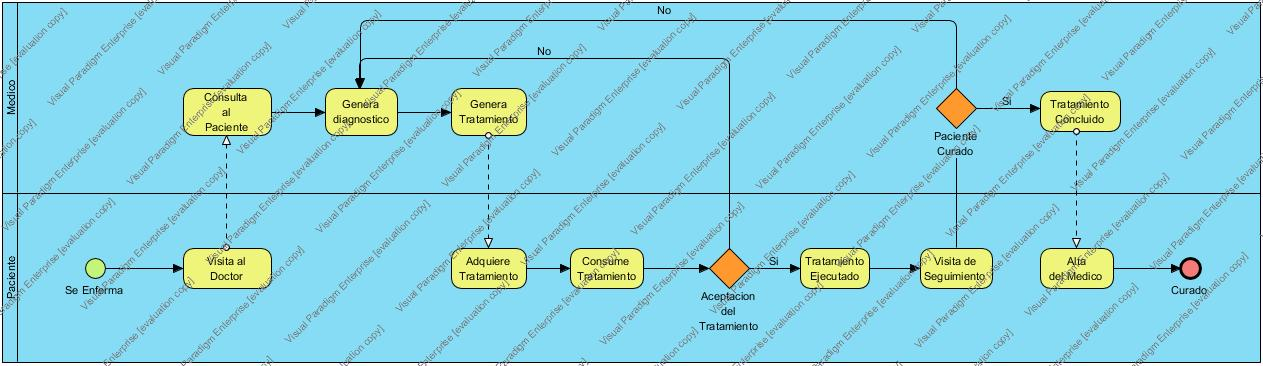
\includegraphics[width=1.1\textwidth]{images/cap2/ProcesoMedico}
	\caption{Proceso medico en la actualidad} \label{fig:proceso1}
\end{figure}

En cambio con el uso de la aplicación como se muestra en la imagen \ref{fig:proceso2} podemos notar como el uso de las nuevas tecnologías ayuda tanto a los pacientes como a los médicos.

\begin{figure}[htb]
	\centering
	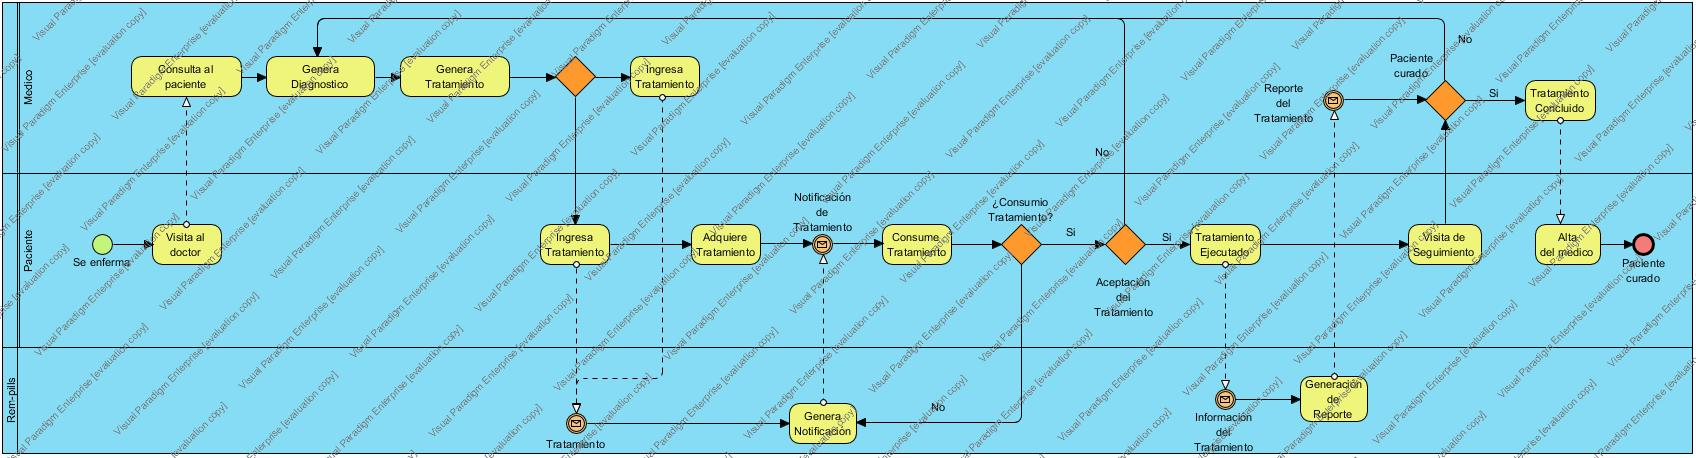
\includegraphics[width=1.1\textwidth]{images/cap2/RemPillstratamiento}
	\caption{Proceso medico en la actualidad} \label{fig:proceso2}
\end{figure}